% !TeX spellcheck = es_ES

\documentclass[10pt,a4paper,titlepage,table]{report}
\usepackage[utf8]{inputenc}
\usepackage[T1]{fontenc}
\usepackage[spanish]{babel}
\usepackage{amsmath}
\usepackage[dvipsnames, table, svgnames]{xcolor}
\usepackage{amsfonts}
\usepackage{amssymb}
\usepackage{graphicx}
\usepackage{pgfplots}
\usepackage{booktabs}

% Change captions font size
\usepackage[font=footnotesize,labelfont=bf]{caption}

% Tweak TOC
% Add dots after sections
\usepackage{tocloft}
\renewcommand{\cftchapleader}{\cftdotfill{\cftdotsep}}

\usepackage{tocbibind} % to add contents and tables of figures and tables in the ToC

% Hyphenation definitions
\hyphenation{de-ve-lop-ment}

% Prevent orphan headers
\usepackage[nobottomtitles]{titlesec}

% Typography refinements
\usepackage{microtype}

% Remove PDF version warnings
%\pdfminorversion=7

% define theorem
\usepackage{mdframed}
\newmdtheoremenv{thm}{Theorem}

% define quotes
\newcommand{\chapquote}[3]{\begin{quotation} \textit{#1} \end{quotation} \begin{flushright} - #2, \textit{#3}\end{flushright} }

% modulus dependencies
\usepackage{subcaption,siunitx,booktabs}
\usepackage{multirow}
\usepackage{tabularx,booktabs}
%\usepackage{apalike}
\usepackage{scrextend}
\usepackage{tablefootnote}
\usepackage{url}
\def\UrlBreaks{\do\/\do-}
\usepackage{breakurl}
% Hide squares around links and break links in different lines if necessary
\usepackage[breaklinks,hidelinks]{hyperref}
\usepackage{makecell}
% distillation dependencies
\usepackage{adjustbox}
% Format titlepage date
\usepackage{datetime}
\usepackage{fancyhdr}

% Define style of the content previous to the chapters
\pagestyle{fancy}
\fancypagestyle{Preamble}{%
	\fancyhead{} %Clean headers
	\fancyhead[LO]{\slshape\nouppercase{\leftmark}}
	\fancyhead[LE]{\thepage}
	\fancyhead[RE]{}
	\fancyhead[RO]{\thepage}
	\fancyfoot{} %Clean headers
	\renewcommand{\chaptermark}[1]{\markboth{\MakeUppercase{ {##1}}}{}}
}

% Define the content of the body
\pagestyle{fancy}
\fancypagestyle{MyStyle}{%
	\fancyhead{} %Clean headers
	\fancyhead[LO]{\slshape\nouppercase{\leftmark}}
	\fancyhead[LE]{\thepage}
	\fancyhead[RE]{\ifnum\value{chapter}=0\else\chaptername\ \thechapter\ \fi}
	\fancyhead[RO]{\thepage}
	\fancyfoot{} %Clean headers
	\renewcommand{\chaptermark}[1]{\markboth{\MakeUppercase{ {##1}}}{}}
}

% Remove the header in the chapter pages
\fancypagestyle{plain}{%
	\renewcommand{\headrulewidth}{0pt}%
	\fancyhf{}%
}

% Add column type Y for distillation paper
\newcolumntype{Y}{>{\centering\arraybackslash}X}


% Configure the bibliography
%\DeclareUnicodeCharacter{0301}{*************************************}
\usepackage[backend=biber, style=apa, natbib=true]{biblatex}
\addbibresource{bibliography.bib} %Imports bibliography file

\author{Iván Vallés Pérez}
\title{Contributions and applications around low resource deep learning modeling}
\newdateformat{monthyeardate}{%
\monthname[\THEMONTH], \THEYEAR}

\begin{document}
	
\makeatletter
\begin{titlepage}

	\begin{figure}[t]
		\centering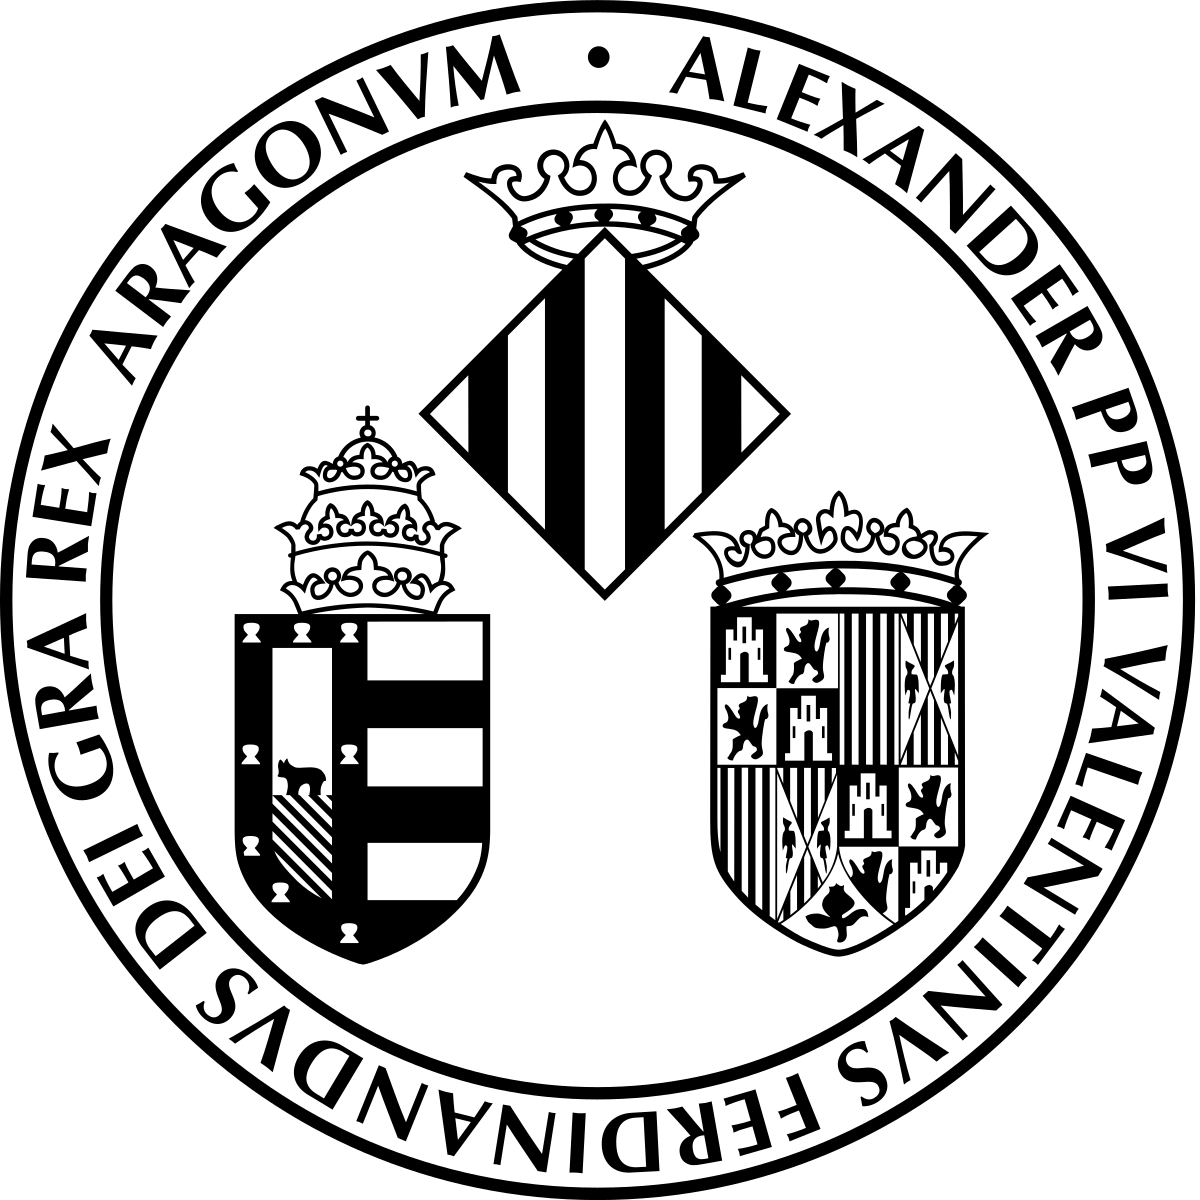
\includegraphics[width=0.5\textwidth]{titlepage/images/logo}
	\end{figure}
	
	\begin{center}
	\textsc{ \LARGE{Universitat de València \\}}
	\textsc{ \LARGE{Escola Tècnica Superior d'Enginyeria \\ }}
	\vspace{5mm}
	{\textsc{PhD Thesis. Doctorat en Enginyeria Electrònica}\\}
	\vspace{40mm}
	\LARGE{\textbf{\@title}}\\ \\
	{\large by Iván Vallés-Pérez \\}
	\vspace{40mm}
	\textnormal{Supervisor: Emilio Soria-Olivas, PhD \\ }
	\textnormal{València - \monthyeardate\today }
	\end{center}

\end{titlepage}
\makeatother

\pagestyle{MyStyle}

\section*{Introducción}
Los algoritmos de aprendizaje profundo representan el estado de la cuestión en lo que a aprendizaje automático se refiere. Muchas de sus aplicaciones requieren una gran cantidad de recursos computacionales, la cual limita su uso a dispositivos de alto rendimiento. El objetivo principal de esta tesis es estudiar métodos y algoritmos que permitan abordar problemas de aprendizaje profundo cuando se tienen recursos computacionales limitados. Este trabajo también tiene como objetivo presentar aplicaciones de aprendizaje profundo en la industria.

En este trabajo se presentan un total de cinco contribuciones al estado del arte del campo del aprendizaje profundo aplicado a problemas que precisan de \textit{hardware} de baja potencia, tales como teléfonos inteligentes, asistentes de voz, televisores inteligentes u otras máquinas de bajo rendimiento. Estas contribuciones proponen o bien una serie de mejoras de los métodos usados comúnmente, o bien una serie de aplicaciones que demuestran la posibilidad de usar este tipo de tecnología sin requerir de un sistema distribuido con muchas máquinas. Cada capítulo de esta tesis presenta una contribución, siendo los capítulos 1 y 2 introductorios y el capítulo 8 un resumen de las conclusiones de cada una de las contribuciones descritas. En este resumen, por razones de brevedad, solo se va a describir el contenido de los capítulos 3 al 7, ambos inclusive.  Por la misma razón, se omiten en este resumen las referencias bibliográficas. Estas se pueden encontrar en la memoria de esta tesis doctoral.


\section*{Contribución 1: el módulo como función de activación}
Esta contribución consiste en el diseño y estudio de una nueva función de activación para redes de aprendizaje profundo: la función \textit{módulo}, $f(x) = |x|$. Esta función de activación tiene una serie de ventajas frente a las demás alternativas. A continuación se detallan las más importantes.

\begin{itemize}
	\item El módulo es una operación de bit, es decir, sólo se requiere un bit para implementarla. Nótese que la función puede expresarse como $f(x) = sgn(x) \cdot x$, donde $sgn(x)$ es la función signo aplicada sobre la variable $x$, y la función signo solo ocupa un único bit. Esto hace a esta función equivalente a la función \textit{ReLU} en términos computacionales.
	\item El módulo es una sencilla operación lineal a trozos, lo cual facilita el cálculo de su derivada, haciendo que su cómputo en tiempo de entrenamiento sea eficiente. La derivada del módulo es $f'(x) = sgn(x)$, por lo que en tiempo de entrenamiento, durante la propagación hacia delante, se pueden guardar los signos de las salidas para ser usados en la fase de \textit{retropropagación}, sin necesidad de ocupar mucha memoria. 
	\item La derivada de la función módulo tiene norma 1 para cualquier valor de $x$, lo cual es ventajoso en diferentes aspectos: (1) los problemas de desvanecimiento de gradiente, observados en las funciones de activación con regiones asintóticas horizontales desaparecen por construcción en el caso del módulo, ya que el gradiente nunca es cercano a cero, (2) por la misma razón que en el punto 1, los problemas de muerte de neuronas observado en funciones de activación tipo \textit{ReLU}, donde se tiene una región 0, no ocurren con el módulo, (3) la derivada de la función, curiosamente, no depende del módulo de $x$, haciendo que la optimización de la red neuronal sea más estable (no van a aparecer gradientes con norma mayor que 1).
\end{itemize}
 
 
Para estudiar el rendimiento de la función de activación propuesta, se plantea compararla con 7 funciones de activación publicadas en otros estudios: \textit{ReLU}, \textit{Leaky ReLU}, \textit{Tanh}, \textit{ELU}, \textit{Swish}, \textit{PFLU} y \textit{Mish}. Dicha comparación se realiza mediante el entrenamiento de 4 arquitecturas distintas de red neuronal, que se entrenan para resolver 3 tareas clásicas de clasificación de imágenes usando los siguientes conjuntos de datos: \textit{MNIST}, \textit{CIFAR10}, \textit{CIFAR100}. Cada experimento se repite 30 veces con distintas inicializaciones de pesos aleatorias para estudiar la significancia estadística de los resultados. A través de los experimentos realizados se observa que la función de activación propuesta mejora los resultados de todas las demás funciones de activación en 75\% de los experimentos realizados. 

Como estudio adicional, y con el objetivo de estudiar el efecto de que la función módulo no sea suave (su derivada no está definida cuando $x=0$) se repiten los experimentos con dos aproximaciones suaves: la tangencial, que usa la función tanh como aproximación a la función $sgn(x)$, y la cuadrática, que usa técnicas de lógica borrosa para combinar la función módulo con la función cuadrática. Se observan resultados en la misma dirección, superando significativamente los resultados de la función módulo original en el 42\% de los casos.

\section*{Contribución 2: destilando el conocimiento de modelos pre-entrenados}
En segundo lugar, se presenta un nuevo método para combinar modelos pre-entrenados usando \textit{técnicas de destilación de conocimiento}. Actualmente se dispone de una gran librería de pesos de modelos que se han pre-entrenado para resolver tareas de ámbito general. Por ejemplo, existe una colección de modelos públicos entrenados para resolver la tarea \textit{ImageNet}, un problema que consiste en aprender a clasificar imágenes a color en 1000 categorías distintas a partir de más de 10 millones de imágenes debidamente etiquetadas. 

Como puede intuirse, entrenar estos modelos requiere de mucho tiempo, energía y \textit{hardware} capaz de realizar esta tarea. La presente contribución se centra en transferir el conocimiento de varios de estos modelos pre-entrenados grandes (llamados modelos profesores), en modelos pre-entrenados más pequeños, de modo que se puedan usar clasificadores de imágenes muy potentes con un bajo coste computacional. Para realizar dicha transferencia de conocimiento entre modelos se usan las técnicas conocidas como técnicas de destilación del conocimiento, que consisten, en resumen, en entrenar los modelos estudiantes sobre las predicciones de los modelos profesores.

Para este estudio se han seleccionado un total de 11 modelos profesores (que se han agrupado en grupos de "el mejor", "los tres mejores" y "todos", según su rendimiento sobre un conjunto de validación), y 4 estudiantes distintos. Adicionalmente, se han definido 5 métodos para la combinación de los profesores: la media, mediana, selección aleatoria, selección de modelo con menor entropía de \textit{Shannon}, o selección del modelo con mayor correlación con el resto de modelos. Se han entrenado 5 modelos con semillas aleatorias distintas para cada uno de los estudiantes, grupo de profesores y método de combinación de profesores. Los resultados de estos experimentos muestran que el uso de las técnicas propuestas permite aumentar significativamente el desempeño de los modelos pre-entrenados más pequeños, lo cual proporciona mejoras computacionales y de rendimiento, reduciendo el número de operaciones de coma flotante hasta en $44.8\times$. 

Como observación final, este trabajo concluye con la siguiente hipótesis. Los modelos pre-entrenados con las técnicas habituales toadavía no han llegado a su máxima capacidad de aprendizaje, puesto que mediante el uso de las técnicas descritas en este capítulo se concluye que el rendimiento de dichos modelos todavía tiene rango de mejora. Esta observación motiva la investigación y el desarrollo de mejores técnicas de entrenamiento para los modelos de aprendizaje profundo



\section*{Contribución 3: sistema integral de predicción de ventas con modelos de aprendizaje profundo}
La tercera aportación de esta tesis aborda el problema de la predicción de ventas en el campo de la logística. Este es un problema importante en la industria de las cadenas de suministro, ya que permite a estos negocios planificar adecuadamente el tráfico en sus almacenes, la mano de obra necesaria y sus relaciones con las compañías de transporte. Junto con una correcta ejecución de los equipos operacionales, la predicción de la demanda de los clientes de un negocio hace posible la orquestación a escala de la logística, lo cual es esencial para el suministro de bienes en un mundo con una población tan elevada como la actual, y con una creciente transición digital.

Para el desarrollo de la solución propuesta se usa un conjunto de datos con los registros de ventas diarias de una compañía llamada \textit{Corporación Favorita} que sita en Ecuador. Este conjunto de datos resume el número de ventas de 4400 productos distintos, en cada uno de sus 54 puntos de venta, entre enero de 2013 y agosto de 2017 (4 años y medio). Además del número de productos vendidos, se tiene información de promociones, detalles cada uno de los puntos de venta y de los productos, el precio del combustible en Ecuador, y las fechas vacacionales globales, regionales y locales. No se tiene información del inventario disponible en cada punto de venta, por lo que la estimación de demanda está sesgada: las ventas representan una cota inferior de la demanda, ya que cuando no hay existencias de un producto no se puede producir una venta. La tarea estudiada en este capítulo consiste en la predicción de las ventas de los siguientes 16 días desde cualquier instante temporal para cualquier producto o punto de venta. Esta decisión no ha sido arbitraria, pues se ha diseñado acorde con los estudios encontrados en la bibliografía, de modo que los resultados sean lo más comparables posible. 

Para resolver este problema, se proponen el estudio de dos sistemas candidatos basados en dos técnicas diferentes de aprendizaje profundo (modelos de secuencia-a-secuencia y \textit{transformers}). Los modelos secuencia-a-secuencia, pese a no ser posible su paralelización a la hora de entrenar, requieren de mucha menos memoria y número de operaciones que los modelos \textit{transformer}. En cambio, se ha observado que los modelos \textit{transformer} proporcionan mejores resultados en distintos campos como visión computacional, procesado de lenguaje natural o habla computacional. Pese a que esta tesis doctoral tiene como objetivo el estudio de técnicas de bajos recursos, se ha incluido el estudio del \textit{transformer} para entender el potencial de mejora de los modelos de secuencia-a-secuencia. 

En ambos casos se propone una solución integral, es decir, un modelo único capaz de predecir las ventas de todos los productos, puntos de venta e instantes temporales. Esto también tiene beneficios computacionales que cabe destacar, dado que, frente a la solución de tener modelos independientes para cada producto o punto de venta, requiere de un solo proceso de búsqueda de hiperparámetros. Además, dada la simplicidad de la solución propuesta, el modelo puede ser implementado en una simple máquina, sin necesidad de usar grandes sistemas complejos en la nube. 

De los resultados de este capítulo se concluye que es posible construir sistemas integrales para la predicción de ventas de múltiples productos, en múltiples puntos de venta y en diferentes momentos en el tiempo, mediante el uso de un único modelo de aprendizaje automático. Más específicamente, se ha observado que, en contra de la intuición inicial, los modelos de secuencia-a-secuencia obtienen mejores resultados que los \textit{transformers}. Además, el estudio de ablación incluido concluye que pese a disponer de las series temporales de las ventas de los casi 5 años, solo se necesitan las ventas de los últimos 75 días para predecir las ventas futuras. Los resultados del modelo propuesto superan significativamente a las alternativas encontradas en la literatura.

\section*{Contribución 4: sistema de detección de comandos de voz mediante el uso de convoluciones eficientes}

Tanto esta contribución como la siguiente pertenecen al campo de la tecnología del habla. En esta contribución se estudia cómo construir un sistema de detección de comandos de voz (conocido como \textit{Keyword Spotting}, en inglés) utilizando una versión eficiente de una red neuronal convolucional. Los sistemas de reconocimiento del habla son cruciales hoy en día, especialmente en asistentes de voz, pero también en sistemas de asistencia a personas con discapacidades auditivas, en entornos donde se requiere atención visual (por ejemplo en automóviles), en centros de telefonía donde se requiere transcribir llamadas de clientes para la posterior explotación de datos o la trazabilidad de experiencia de usuario. 

Muchas de las soluciones actuales requieren de la asistencia de potentes ordenadores en la nube. En este caso particular, esto tiene múltiples desventajas frente a un sistema integrado en el dispositivo.

\begin{itemize}
	\item La comunicación con un servidor en la nube está sujeta a una latencia, la cual tiene un efecto directo en la experiencia de usuario.
	\item El uso de un servidor en la nube requiere que tanto los comandos de voz como su transcripción se transmitan a través de Internet, y que en algunos casos incluso se almacenen en el servidor durante un tiempo. Esto comúnmente suscita preocupación en los clientes con respecto a su privacidad. 
	\item Un servidor en la nube normalmente requiere mucha más energía que un dispositivo integrado.
\end{itemize}

Para este estudio se usa un conjunto de datos llamado \textit{Google tensorflow speech-commands dataset} el cual se distribuye en dos versiones (V1 y V2). Este consta de un conjunto de grabaciones etiquetado, de un segundo de duración, de palabras que se corresponden con los distintos comandos de voz a detectar. Se dispone de 64.721 y de 105.829 clips de audio en las versiones V1 y V2, respectivamente. Entre estas grabaciones hay 30 (en la versión V1) o 35 (en la versión V2) comandos distintos. Los distintos comandos de voz registrados por los locutores se corresponden con las siguientes palabras: ``left'', ``right'', ``yes'', ``no'', ``down'', ``up'', ``go'', ``stop'', ``on'', ``off'', ``zero'', ``one'', ``two'', ``three'', ``four'', ``five'', ``six'', ``seven'', ``eight'', ``nine'', ``dog'', ``cat'', ``wow'', ``house'', ``bird'', ``happy'', ``sheila'', ``marvin'', ``bed'', ``tree'', ``visual'', ``follow'', ``learn'', ``forward'', ``backward''. Estos clips de audio están registrados con una frecuencia de muestreo de 16kHz.

Con el objetivo de comparar con los estudios encontrados en la literatura, se agrupan estos comandos en grupos de 35 comandos, 20 comandos, 10 comandos y 2 comandos, definiendo un total de 4 tareas a resolver. En cada caso, los comandos no correspondientes con cada tarea se agrupan en una nueva clase llamada ``unknown'' (desconocido), la cual representará una clase extra en las tareas de clasificación. Además, cada clip de audio se distorsiona (mediante la combinación aleatoria de varios tipos de transformaciones de la señal: cambio de frecuencia, remuestreo, adición de ruido, corte, etc) generando 5 nuevas versiones de las grabaciones originales, que se combinan con los datos originales sin distorsionar para entrenar el modelo.

Se diseña una arquitectura basada en redes convolucionales separables en profundidad (\textit{depthwise separable convolutions}, en inglés), la cual está basada en una arquitectura comunmente usada en tareas de visión computacional, bautizada como \textit{Xception}. Este tipo de convoluciones se diferencia de la operación original en que separa la computación de los canales de la computación espacial, lo cual hace que sea sustancialmente más eficiente. 

Para estudiar el desempeño de esta nueva arquitectura se entrena el modelo neuronal propuesto 5 veces, con inicializaciones aleatorias distintas, de modo que se pueda calcular la significancia estadística de los resultados obtenidos. Además, a modo de punto de comparación adicional, cuatro sujetos etiquetaron 1000 comandos aleatorios manualmente. Los resultados de este experimento demuestran que el sistema propuesto no solo es capaz de superar el rendimiento de las alternativas en la literatura, sino que en dos de las cuatro tareas es capaz de superar el rendimiento humano significativamente. 
	
\section*{Contribución 5: sistema de generación de habla de múltiples perfiles de voz}
El último estudio propone el diseño y estudio de un modelo independiente de generación de habla capaz de sintetizar voz natural e inteligible usando miles de perfiles de voz distintos. La generación del habla es, al igual que el reconocimiento del habla (la tarea opuesta), una importante aplicación en diferentes escenarios: asistentes de voz, asistencia a personas con discapacidades visuales, asistencia en actividades que requieren concentración visual tales como la conducción, el ocio (por ejemplo la lectura de noticias mientras el usuario realiza cualquier acción, etc). A diferencia de la tarea de reconocimiento del habla, esta es una tarea generativa: no hay una única forma de leer una frase. Por lo tanto, el modelo generativo tiene que ser capaz de generar voces usando distintos perfiles de voz, además de modelar correctamente las distintas variaciones prosódicas de cada frase. Si el modelo no es capaz de modelar esta variabilidad, las voces sintéticas no serán naturales, lo cual empeorará la experiencia de usuario.

Este estudio parte de una de las arquitecturas más conocidas en el campo de generación del habla bautizada como \textit{Tacotron}. Esta arquitectura cuenta con dos módulos: un codificador y un decodificador. El codificador recibe como entrada el texto que se quiere leer, un vector latente representando el perfil de voz deseado, así como una referencia acústica de donde se extrae la información prosódica que se quiere implantar en la síntesis. El decodificador es un módulo autoregresivo que se usa para generar el espectrograma con la información acústica deseada. El alineamiento de la información acústica y la léxica se consigue mediante el uso de un mecanismo de atención. 

Sobre esta arquitectura se proponen los siguientes cambios.

\begin{itemize}
	\item Se sustituye el codificador de la referencia acústica por un \textit{auto-encoder variacional}, el cual es responsable de modelar las distintas formas de leer una frase dada. De este modo, aparte de mejorar la generalización del modelo se elimina la dependencia en un sistema de generación suplente en tiempo de inferencia. 
	\item Se normaliza el vector latente correspondiente con el perfil de voz deseado usando técnicas de flujos de normalización. Estos se usan de modo que el espacio latente donde se hallan las representaciones de los perfiles de voz se distribuya de acuerdo a una distribución normal $\mathcal{N}(0, I)$.
\end{itemize}

Se entrenan ambos sistemas, en igualdad de condiciones, usando un conjunto de datos consistente en más de 700.000 clips de audio grabados por alrededor de 3000 distintos locutores. Estos clips de audio están registrados con una frecuencia de muestreo de 16kHz.

Una vez entrenado el sistema, se realizan los siguientes experimentos 

\begin{enumerate}
	\item Con cada uno de los sistemas, se sintetizan 50 frases para cada uno de los perfiles de voz disponibles (2870) y se estudia su inteligibilidad (mediante la comparación de la frase objetivo y la transcripción automática del audio generado) y cómo de distintos son entre ellos (mediante el uso de un modelo de verificación del locutor).
	\item Se realiza una síntesis repetida (con distintas semillas aleatorias) de una serie de frases para determinar la capacidad de cada sistema de modelar la prosodia. Para ello se miden una serie de variables cuantitativas sobre las síntesis, que representan aspectos relacionados con la prosodia (por ejemplo la frecuencia fundamental).
	\item Se estudia cómo los sistemas reaccionan ante perfiles de voz sintéticos obtenidos mediante la interpolación lineal de sus representaciones latentes.
\end{enumerate}

Los resultados de los experimentos descritos concluyen que el modelo propuesto es capaz de generar habla expresiva con mayores variaciones de prosodia significativas, con respecto al modelo base. Además, se prueba empíricamente que ambos modelos tienen el mismo nivel de inteligibilidad y generan voces distintas por igual. El modelo propuesto generaliza mejor ante perfiles de voz interpolados. 

El enfoque propuesto elimina la dependencia de los modelos anteriores de un sistema de voz auxiliar, lo que lo hace más eficiente en el tiempo de entrenamiento e inferencia.

\end{document}


